% !TEX root = MAIN.tex

\chapter{Software product quality assurance}

% a.	The SPAP shall describe the approach taken to ensure the quality of the software product.
% b.	The description of the approach specified in B.2.1<7>a shall include the:
% 1.	specification of the product metrics, their target values and the means to collect them;
% 2.	definition of a timely metrication programme;
% 3.	analyses to be performed on the collected metrics;
% 4.	way the results are fed back to the development team;
% 5.	documentation quality requirements;
% 6.	assurance activities meant to ensure that the product meets the quality requirements.
%

\section{Approach}

In this project, the verification and validation of the different software that compose the \FAQAS (i.e., \MASS, \SEMUS, and \DAMA) is performed at two levels: (1) unit test level, and (2) system test level.

\subsection{Unit Testing}

At this level, we assess the quality of single, encapsulated components. In other words, components that do not interact with other units, but simply store results in files processed by other units.

Given its characteristics, we followed this procedure to assess the component \texttt{SRCMutation} from \MASS, and the component \texttt{DDMutation} from \DAMA.

\subsubsection{MASS: SRCMutation}

\begin{figure}[t]
  \centering
  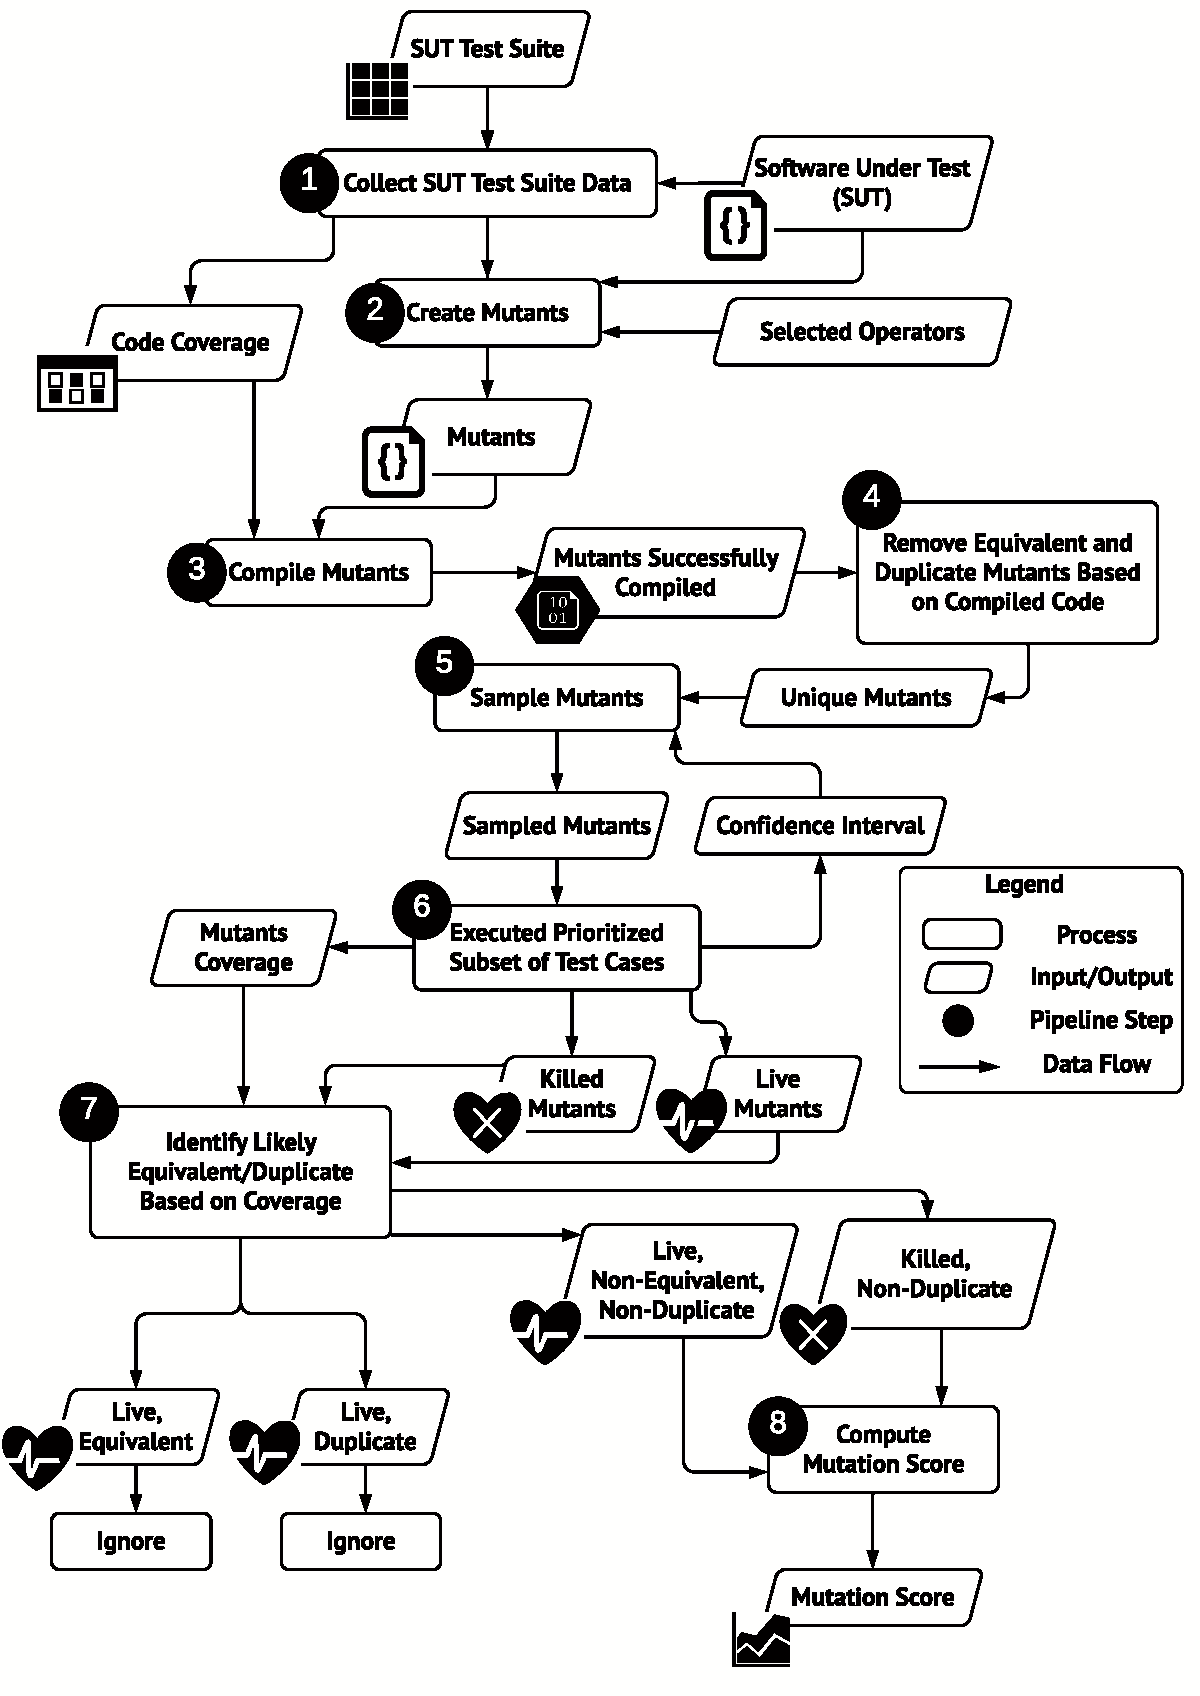
\includegraphics[width=0.6\textwidth]{images/Approach.pdf}
      \caption{MASS methodology.}
      \label{fig:mass}
\end{figure}

Figure~\ref{fig:mass} introduces \MASS methodology. The component \texttt{SRCMutation} is implemented in step 2 of the methodology under the name of \emph{Create Mutants}.

\texttt{SRCMutation} is the component with the most complicate implementation logic and thus it requires a detailed unit testing. All the other components either filter or join data, so their implementation is simpler and thus their test automation is performed through system tests.

For more details, please refer to Chapter 7 of the SUITP document.


\subsubsection{DAMAt: DDMutation}

\begin{figure}[t]
  \centering
  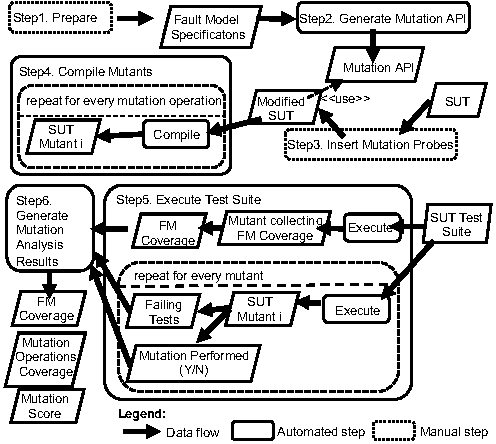
\includegraphics[width=0.6\textwidth]{images/dataDrivenBufferProcess.pdf}
      \caption{DAMAt methodology.}
      \label{fig:damat}
\end{figure}

Figure~\ref{fig:damat} introduces the \DAMA methodology. The component \texttt{DDMutation} is implemented in step 2 of the methodology under the name of \emph{Generate Mutation API}.

\texttt{DDMutation} is the component with the most complicate implementation logic and thus it requires a detailed unit testing. All the other components either filter or join data, so their implementation is simpler and thus their test automation is performed through system tests.

For more details, please refer to Chapter 11 of the SUITP document.

\subsection{System Testing}

At this level, we test the system as a whole. In particular, we verify and validate all the functional requirements specified in the Software System Specifications document (SSS), for the three software systems of the \FAQAS.

\subsubsection{MASS}

At a system level, we validate that \MASS is able to process the SUT, SUT test suite, and perform correctly the following steps (1) collect SUT test suite data (e.g., code coverage information), (2) create mutants, (3) compile mutants, (4) disregard equivalent and duplicate mutants based on compiler optimizations, (5) sample mutants, (6) execute a prioritized subset of test case, (7) identify likely equivalent based on code coverage, and (8) compute the mutation score.

We validated the eight steps of \MASS on the MLFS case study, and verified that outputs complied with the system specifications. A full description of the validation of \MASS can be found on the SUM document on Chapter 11.

\subsubsection{SEMuS}

\begin{figure}[t]
  \centering
  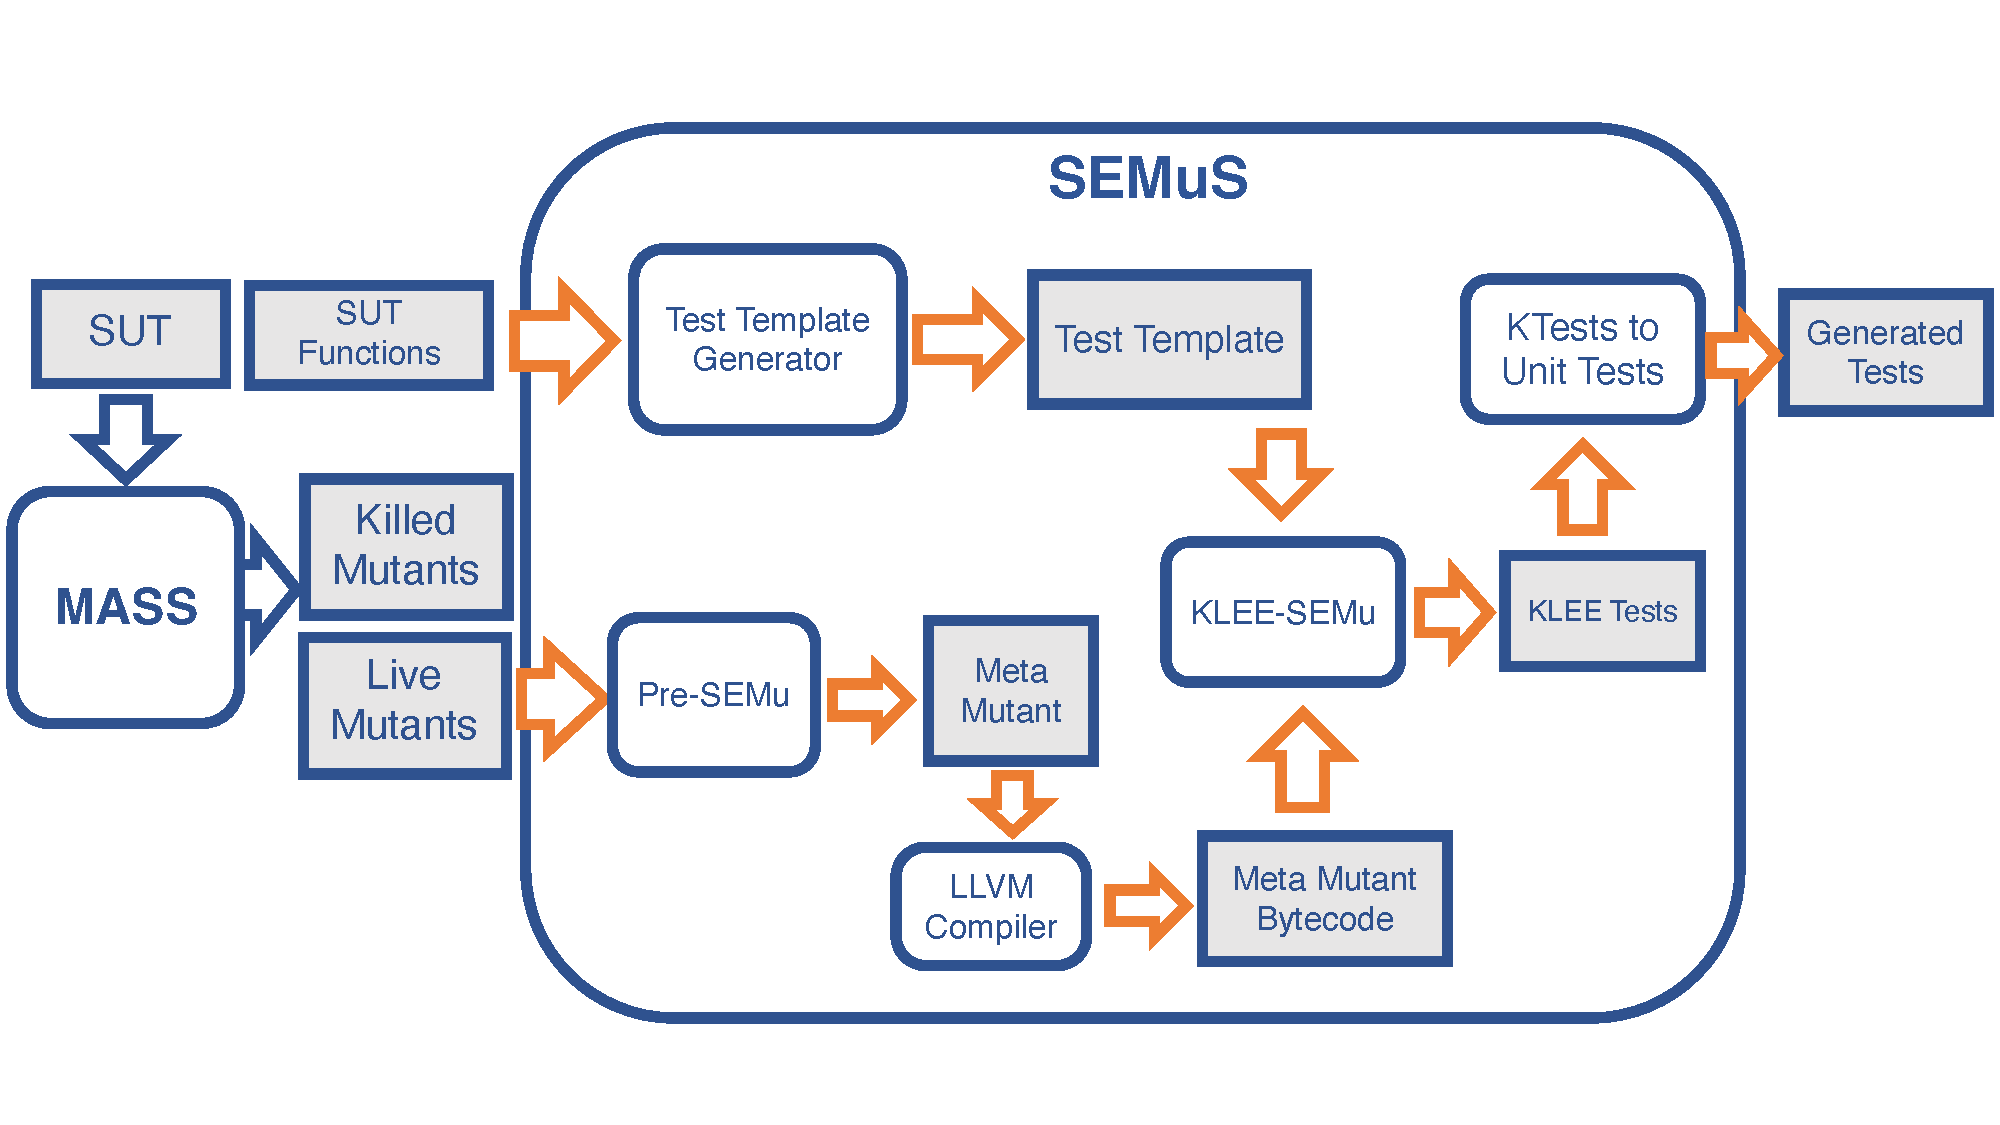
\includegraphics[width=0.8\textwidth]{images/semus-architecture.pdf}
      \caption{SEMuS architecture.}
      \label{fig:semus}
\end{figure}

Figure~\ref{fig:semus} introduces the \SEMUS architecture, and in particular the different inputs and outputs to be considered for verification and validation.

At a system level, we performed a validation of \SEMUS to assure that every functional requirement is compliant with the Software System Specifications document (SSS) document. Particularly, we verified that \SEMUS was able to parse the SUT source code, and perform correctly the following steps (as shown in Figure~\ref{fig:semus}) (1) generate test templates from SUT functions, (2) generate the meta-mutants containing all the live mutants of SUT test suite, (3) compile the meta-mutant and to invoke KLEE-SEMu to trigger the test generation step, and (4) to process the KLEE tests and to convert them to C readable unit test cases.

We validated the four steps of the methodology on the MLFS case study, we also verified that outputs are in line with system specifications. A detailed description of the validation of \SEMUS can be found on the SUM document on Chapter 12.


\subsubsection{DAMAt}

At a system level, we performed a validation of \DAMA to assure that every functional requirement is compliant with the Software System Specifications document (SSS) document.
Particularly, we verified that \DAMA was able to:
\begin{enumerate}
	\item Parse a fault model prepared by the user.
	\item Generate a mutation API with the functions that modify the data according to the provided fault model.
  \item Modify the buffer through calls to the mutation API.
	\item Generate and compile mutants.
	\item Execute the test suite against all the mutants and gather the results of the test cases.
	\item Generate the results of the mutation analysis.
\end{enumerate}

We validated the six steps of the methodology on the following case studies:
\begin{itemize}
  \item LXS System Test Suite for ESAIL
  \item GSL Integration Test Suite for libgscsp
  \item GSL System Test Suite for libparam
\end{itemize}

We also verified that outputs are in line with system specifications. A detailed description of the validation of \DAMA can be found in the D4 document.

\clearpage
